



\chapter{Utilisation du calcul littéral}





\section{Développer et factoriser}
\subsection{Simple et double distributivité}

\begin{Définition}
{\bf{Développer}} un produit signifie écrire ce produit sous la forme d'une somme (ou différence) de termes. \\
{\bf{Factoriser}} une somme signifie écrire cette somme sous forme d'un produit de facteurs.
\end{Définition}

\vspace{0.5cm}

\begin{Propriété}
Soient $a$ et $b$ et $k$ trois réels : 

\begin{center}
\begin{tikzpicture}
% Formule principale
\node at (0,0) { \Large $k(a+b) = \textcolor{Couleur8}{ka} + \textcolor{Couleur3}{kb}$};

% Flèches courbes colorées
% Flèche Couleur8 de k vers ka
\draw[->,>=latex,Couleur8,thick,bend left=30] (-1.9,0.3) to (-1.3,0.3);

% Flèche verte de k vers kb  
\draw[->,>=latex,Couleur3,thick,bend left=50] (-1.9,0.3) to (-0.6,0.3);


\end{tikzpicture}
\end{center}

\end{Propriété}

\vspace{0.5cm}

\begin{Exemple}
\leavevmode\vspace{-\baselineskip}
\begin{itemize}[label=\textcolor{Couleur8}{$\bullet$}]
\item $3(x+1)=3x+3$
\item $7(2y-5)=14y-35$
\item $(-2z^2-1)\times 8z=-16z^3-8z$
\item $-6(t^2-9t)=-6t^2+54t$
\end{itemize}
\end{Exemple}

\vspace{0.5cm}

\begin{Propriété}
Soient $a$, $b$, $c$ et $d$ quatre réels : 
%\begin{large}
%$$(a+b)(c+d)={\color{Couleur8}{a\times c}} + {\color{Couleur6}{a\times d}}+{\color{Couleur8}{b\times c}} + {\color{violet}{b\times d}}$$
%\end{large}
\begin{center}
\begin{tikzpicture}
% Formule principale
\node (formula) at (0,0) {\Large $(a+b)(c+d) = \textcolor{Couleur8}{ac} + \textcolor{Couleur3}{ad} + \textcolor{Couleur6}{bc} + \textcolor{violet}{bd}$};

% Positionnement des termes pour les flèches
\coordinate (a) at (-3.2,0.3);
\coordinate (b) at (-2.5,0.3);
\coordinate (c) at (-2,0.3);
\coordinate (d) at (-1,0.3);

\coordinate (a') at (-3.2,-0.3);
\coordinate (b') at (-2.5,-0.3);
\coordinate (c') at (-2,-0.3);
\coordinate (d') at (-1,-0.3);


% Flèches courbes colorées montrant les produits
% a × c (Couleur8)
\draw[<-,>=latex,Couleur8,thick,bend left=30] (c') to[out=50,in=130] (a');

% a × d (vert)
\draw[<-,>=latex,Couleur3,thick,bend left=20] (d') to[out=40,in=140] (a');


% b × d (violet)
\draw[->,>=latex,violet,thick,bend left=20] (b) to[out=40,in=140] (d);

% b × c (cyan)
\draw[->,>=latex,Couleur6,thick,bend left=30] (b) to[out=50,in=130] (c);


\end{tikzpicture}
\end{center}


\end{Propriété}

\vspace{0.5cm}

\begin{Exemple}
\leavevmode\vspace{-\baselineskip}

\begin{itemize}[label=\textcolor{Couleur8}{$\bullet$}]
\item $(x+1)(2x+5)=2x^2+5x+2x+5=2x^2+7x+5$
\item $(2y-3)(3y+5)=6y^2+10y-9y-15=6y^2+y-15$
\item $(3z-7)(2z-4)=6z^2-12z-14z+28=6z^2-26z+28$
\item $(5t^2-2t)(-3t-4)=-15t^3-20t^2+6t^2+8t=-15t^3-14t^2+8t$
\end{itemize}

\end{Exemple}

\newpage

\subsection{Identités remarquables}

\begin{Théorème}
Soient $a$ et $b$ deux réels alors : 
\vspace{-0.5cm}
\begin{multicols}{3}
\begin{itemize}[label=\textcolor{Couleur1}{$\bullet$}]
\begin{large}
\item $(a+b)^2=a^2+2\times a \times b+b^2$
\item $(a-b)^2=a^2-2\times a \times b+b^2$
\item $(a+b)(a-b)=a^2 - b^2$
\end{large}
\end{itemize}
\end{multicols}
\vspace{0.2cm}
\end{Théorème}

\begin{Exemple}
Développer les expressions suivantes :

\begin{itemize}[label=\textcolor{Couleur8}{$\bullet$}]
\item $(x-5)^2 =x^2 -2\times x\times 5+5^2 = x^2-10x +25$
\item  $(2x-1)(2x+1)=(2x)^2 -1^2 =4x^2 -1$.
\item $(x+3)^2=x^2+2\times x \times 3 +3^2 =x^2 +6x+9$
\end{itemize}


\end{Exemple}

\begin{minipage}[c]{0.6\linewidth}
\begin{proof}
On considère un carré bleu de côté $a$ et d'aire $a^2$, un carré rouge de côté $b$ et d'aire $b^2$, et un carré noire de côté $a+b$ et d'aire $(a+b)^2$. En pavant le carré noire avec le carré bleu et le carré rouge, on peut constater qu'il reste deux rectangles non occupés (vert) de largeur $a$ et de longueur $b$ (donc d'aire $a\times b$). En additionnant les aires correspondantes, on en déduit : $(a+b)^2={\color{Couleur6}{a^2}}+{\color{Couleur11}{b^2}}+2{\color{Couleur8}{ab}}$\\

On a la formule $(a-b)^2=a^2-2\times a \times b+b^2$ en considérant l'autre figure. \\

Par ailleurs, par double distributivité, on a : \\
$(a+b)(a-b)=a^2-ab+ba-b^2=a^2-b^2$.
\end{proof}
\end{minipage} \hfill
\begin{minipage}[c]{0.3\linewidth}

% Figure 2: (a+b)²
\begin{center}
\begin{tikzpicture}[scale=1.2]


% Zones colorées
\fill[Couleur6!30] (0,0) rectangle (2,2);
\fill[Couleur8!30] (2,0) rectangle (3,2);
\fill[Couleur8!30] (0,2) rectangle (2,3);
\fill[Couleur11!30] (2,2) rectangle (3,3);

\draw[Couleur6] (0,0) rectangle (2,2);
\draw[Couleur8] (2,0) rectangle (3,2);
\draw[Couleur8] (0,2) rectangle (2,3);
\draw[Couleur11] (2,2) rectangle (3,3);


% Labels dans chaque zone
\node at (1,1) {\large $a^2$};
\node at (2.5,1) {\large $ab$};
\node at (1,2.5) {\large $ab$};
\node at (2.5,2.5) {\large $b^2$};

% Cotes
\draw[<->] (0,-0.3) -- (2,-0.3) node[midway,below] {$a$};
\draw[<->] (2,-0.3) -- (3,-0.3) node[midway,below] {$b$};
\draw[<->] (-0.3,0) -- (-0.3,2) node[midway,left] {$a$};
\draw[<->] (-0.3,2) -- (-0.3,3) node[midway,left] {$b$};

\end{tikzpicture}
\end{center}


% Figure 1: (a-b)²
\begin{center}
\begin{tikzpicture}[scale=1.2]

% Hachures pour les zones à soustraire
\fill[pattern=north east lines, pattern color=Couleur8!50] (0,0) rectangle (1,1);
\fill[pattern=north east lines, pattern color=Couleur8!50] (1,0) rectangle (3,1);
\fill[pattern=north east lines, pattern color=Couleur8!50] (0,1) rectangle (1,3);

% Hachures pour les zones à soustraire
\draw[Couleur8!50] (0,0) rectangle (1,1);
\draw[Couleur8!50] (1,0) rectangle (3,1);
\draw[Couleur8!50] (0,1) rectangle (1,3);

% Zone principale colorée
\fill[Couleur2!30] (1,1) rectangle (3,3);
\draw[Couleur2] (1,1) rectangle (3,3);

% Labels
\node at (2,2) {\large $(a-b)^2$};

% Cotes
\draw[<->] (0,-0.3) -- (1,-0.3) node[midway,below] {$b$};
\draw[<->] (0,-0.7) -- (3,-0.7) node[midway,below] {$a$};
\draw[<->] (-0.3,0) -- (-0.3,1) node[midway,left] {$b$};
\draw[<->] (-0.7,0) -- (-0.7,3) node[midway,left] {$a$};

\end{tikzpicture}
\end{center}

\end{minipage} 

\begin{Méthode}Développer une expression\\
Développer, réduire et ordonner l'expression suivante : 
$A=(x+2)(4x-3)-x(7-x)^2$.
On a : 
\begin{align*}
A&=4x^2-3x+8x-6-x(7^2-2\times 7 \times x+x^2)\\
&=4x^2+5x-6-x(49-14x+x^2)\\
&=4x^2+5x-6-49x-14x^2-x^3\\
&=-x^3-10x^2-44x-6
\end{align*}
\end{Méthode}

\newpage

\subsection{Factoriser}

\noindent Pour factoriser, il faut trouver dans chacun des termes de l'expression un {\textcolor{Couleur8}{facteur commun}}.

\begin{Méthode}Factoriser une expression \\
Factoriser les expressions suivantes :\\
${\color{Couleur6}{\bullet}}B = 3(2 + 3x) - (5 + 2x)(2 + 3x)$ \quad ${\color{Couleur6}{\bullet}}C=(2-5x)^2 -(2-5x)(1+x)$ \quad $ {\color{Couleur6}{\bullet}}D = 5(1 - 2x) - (4 + 3x)(2x - 1)$ \quad $ {\color{Couleur6}{\bullet}}E=3x^2 -x$

\begin{multicols}{2}
\begin{align*}
B&={\color{Couleur6}{3}}{\color{Couleur8}{(2 + 3x)}} {\color{Couleur6}{- (5 + 2x)}}{\color{Couleur8}{(2 + 3x)}}\\
&={\color{Couleur8}{(2 + 3x)}}{\color{Couleur6}{(3- (5 + 2x))}}\\
&=(2+3x)(3-5-2x)\\
&=(2+3x)(-2-2x)
\end{align*}

\begin{align*}
C&={\color{Couleur8}{(2-5x)}}{\color{Couleur6}{(2 - 5x)}} {\color{Couleur6}{-}}{\color{Couleur8}{(2-5x)}}{\color{Couleur6}{(1+x)}}\\
&={\color{Couleur8}{(2 -5x)}}{\color{Couleur6}{((2-5x)- (1+x))}}\\
&=(2-5x)(2-5x-1-x)\\
&=(2-5x)(1-6x)
\end{align*}
\end{multicols}

\begin{multicols}{2}
\begin{align*}
D&=5(1-2x){\color{Couleur3}{-}}(4+3x){\color{Couleur3}{(2x-1)}}\\
&=5(1-2x){\color{Couleur3}{+}}(4+3x){\color{Couleur3}{(1-2x})}\\
&={\color{Couleur8}{(1-2x)}}{\color{Couleur6}{(5+(4+3x))}}\\
&=(1-2x)(9+3x)
\end{align*}

\begin{align*}
E&=3x^2-x\\
&=3x^2-x{\color{Couleur3}{\times 1}}\\
&={\color{Couleur8}{x}}{\color{Couleur6}{(3x-1)}}\\
\end{align*}
\end{multicols}


\end{Méthode}

\begin{Méthode}Factoriser en utilisant une identité remarquable \\
Factoriser les expressions suivantes :
${\color{Couleur6}{\bullet}}F = 16x^2-40x+25$ \quad ${\color{Couleur6}{\bullet}}G=(3x+1)^2-49$ 

\begin{minipage}[c]{0.5\linewidth}
\noindent Pour $F$ : on reconnaît une identité remarquable du type $a^2-2ab+b^2=(a-b)^2$ avec $a=4x$ et $b=5$.\\
Donc $F=16x^2-40x+25=(4x-5)^2$.\\




\noindent Pour $G$ : on reconnaît une identité remarquable du type $a^2 - b^2 = (a + b)(a - b)$ avec $a=3x+1$ et $ b=7$.
\end{minipage} \hfill
\begin{minipage}[c]{0.4\linewidth}
\begin{align*}
G&=(3x+1)^2 -49 \\
&= {\color{Couleur8}{(3x+1)}}^2- {\color{Couleur6}{7}}^2 \\
&=( {\color{Couleur8}{(3x+1)}}+ {\color{Couleur6}{7}})({\color{Couleur8}{(3x+1)}}- {\color{Couleur6}{7}})\\
&=( (3x+1)+ 7)((3x+1)- 7)\\
&=(3x+8)(3x-6)
\end{align*}
\end{minipage}




\end{Méthode}


\newpage


\section{Équations et inéquations produit et quotient}

\subsection{Équation-produit}

\begin{Définition}
Toute équation du type $P(x) \times Q(x) = 0$, où $P(x)$ et $Q(x)$ sont des expressions algébriques, est appelée {\bf{équation-produit}}.

\end{Définition}


\begin{Propriété} $ $\\
\vspace{-0.5cm}
\begin{itemize}[label=\textcolor{Couleur2}{$\bullet$}]
\item Dire qu'un produit de facteurs est nul, équivaut à dire que l'un au moins des facteurs est nul.
\item Le cas particulier de l'équation-produit $(ax + b)(cx + d) = 0$ équivaut à $ax+b=0$ ou $cx+d=0$.
\end{itemize}
\end{Propriété}



\begin{Méthode}Résoudre une équation en se ramenant à une équation-produit \\
Résoudre dans $\R$ les équations suivantes : 

\begin{enumerate}

\item $(5 + 2x)(2 - 3x)=0$ 
\item $(3x+1)(1-6x)-(3x+7)(3x+1)=0$
\item $ 5x^2-4x=0$

\end{enumerate}
\vspace{0.5cm}
\begin{enumerate}
\item $(5 + 2x)(2 - 3x)=0$ donc soit : \begin{align*}
5+2x=0 & \text{ ou } 2-3x=0 \\
2x=-5 & \text{ ou } -3x=-2 \\
x=\dfrac{-5}{2} & \text{ ou } x=\dfrac{2}{3} \\
\end{align*}

\underline{Vérification} : $5+2\times \dfrac{-5}{2}=5-5=0$ et $2-3\times\dfrac{2}{3}=2-2=0$. Donc $S=\left\{\dfrac{-5}{2} \text{ ; } \dfrac{2}{3}\right\}$

\item On commence par factoriser l'expression pour se ramener à une équation-produit :\\

\begin{minipage}[c]{0.45\linewidth}
\begin{align*}
&(3x + 1)(1 - 6x) - (3x + 7)(3x + 1) = 0 \\
&(3x + 1)[(1 - 6x) - (3x + 7)] = 0\\
&(3x + 1)(1 - 6x -3x - 7) = 0\\
&(3x + 1)(- 9x - 6) = 0
\end{align*}
\end{minipage} \hfill
\begin{minipage}[c]{0.45\linewidth}
\begin{align*}
\text{ Soit } 3x + 1 = 0 &\text{ ou } - 9x - 6 = 0\\
3x = -1 &\text{ ou } - 9x = 6\\
x=\dfrac{-1}{3} &\text{ ou } x=\dfrac{6}{-9}=\dfrac{-2}{3}
\end{align*}

\end{minipage}
\underline{Vérification} : $\left(3\times \dfrac{-1}{3} + 1\right)\left(1 - 6\times \dfrac{-1}{3}\right) - \left(3\times \dfrac{-1}{3} + 7\right)\left(3\times \dfrac{-1}{3} + 1\right) =0$ et \\$\left(3\times \dfrac{-2}{3} + 1\right)\left(1 - 6\times \dfrac{-2}{3}\right) - \left(3\times\dfrac{-2}{3} + 7\right)\left(3\times \dfrac{-2}{3} + 1\right) = 0$. Donc $S=\left\{\dfrac{-1}{3} \text{ ; } \dfrac{-2}{3}\right\}$
\vspace{0.2cm}
\item On commence par factoriser l'expression pour se ramener à une équation-produit :\\
\vspace{-0.2cm}
\begin{minipage}[c]{0.45\linewidth}
\begin{align*}
5x^2-4x&=0\\
x(5x-4)&=0
\end{align*}
\end{minipage} \hfill
\begin{minipage}[c]{0.45\linewidth}
\begin{align*}
\text{ Soit } x = 0 &\text{ ou } 5x-4 = 0 \\
 &\text{ ou } 5x = 4\\
&\text{ ou } x=\dfrac{4}{5}
\end{align*}
\end{minipage}

\underline{Vérification} : $5\times 0^2-4\times 0=0$ et $5\times \dfrac{4}{5}^2-4\times \dfrac{4}{5} = \dfrac{20}{25}-\dfrac{20}{25}=0$. Donc $S=\left\{0 \text{ ; } \dfrac{4}{5}\right\}$\\
~\\
\end{enumerate}


\end{Méthode}

\newpage

\subsection{Équations quotient}

\begin{Définition}
Toute équation du type $\dfrac{P(x)}{Q(x)} = 0$, où $P(x)$ et $ Q(x)$ sont des expressions algébriques (avec $Q(x) \neq 0$), est appelée équation-quotient.
\end{Définition}

\begin{Propriété}
Pour tout $x$ qui n'annule pas l'expression $Q(x)$, l'équation-quotient $\dfrac{P(x)}{Q(x)}= 0$ équivaut à $P(x) = 0$.

\end{Propriété}

\begin{Exemple}
Résoudre dans $\R$ les équations suivantes :
\begin{enumerate}
\item $\dfrac{x+2}{x+3} = 0 $. L'équation n'est pas définie pour $x = -3$.\\Pour $x\neq -3$, l'équation $\dfrac{x+2}{x+3} = 0 $ équivaut à $x+2=0$. D'où $x=-2$, $S=\left\{-2\right\}$.
~\\
\item $\dfrac{3x+5}{x-1}=0$ .
L'équation n'est pas définie pour $x = 1$.\\
Pour $x\neq 1$, l'équation $\dfrac{3x+5}{x-1} = 0 $ équivaut à $3x+5=0$. D'où $x=\dfrac{-5}{3}$, $S=\left\{\dfrac{-5}{3}\right\}$.
~\\
\item $\dfrac{(2x+1)(x-3)}{x-4}=0$ .
L'équation n'est pas définie pour $x = 4$. \\
Pour $x\neq 4$, l'équation $\dfrac{(2x+1)(x-3)}{x-4} = 0 $ équivaut à $(2x+1)(x-3)=0$. Soit $2x+1=0$ ou $x-3=0$.\\
Donc $S=\left\{-\dfrac{1}{2} \text{ ; } 3\right\}$.
~\\
\item $\dfrac{x^2-9}{x+3}$ .
L'équation n'est pas définie pour $x = -3$.\\
Pour $x\neq -3$, l'équation $\dfrac{x^2-9}{x+3} = 0 $ équivaut à $x^2-9=0$. D'où $x=3$ ou $x=-3$, ainsi, $S=\{-3\text{ ; } 3\}$.
\end{enumerate}

\end{Exemple}
\newpage
\subsection{Inéquations produit et quotient}

\begin{Méthode}Résoudre une inéquation en étudiant le signe d'un produit \\
Résoudre dans $\R$ l'inéquation suivante : $(3-6x)(x+2)>0$\\
Le signe de $(3 - 6x)(x + 2)$ dépend du signe de chaque facteur $3 - 6x$ et $x + 2$
\begin{align*}
3-6x=0 &\text{  ou  } x+2=0 \\
6x=3 &\text{  ou  } x=-2 \\
x=\dfrac{3}{6}=\dfrac{1}{2}
\end{align*}
Résumons dans un même tableau de signes les résultats pour les deux facteurs. En appliquant la règle des signes, on en déduit le signe du produit $(3-6x)(x + 2)$.\\
\begin{minipage}[c]{0.45\linewidth}
\begin{tikzpicture}
      \tkzTabInit[espcl=1.5,lgt=3]{$x$ /1  , $3-6x$ /0.7 , $x+2$ /0.7 , $(3-6x)(x+2)$ /0.7} { $-\infty$ , $-2$ , $\dfrac{1}{2}$, $+\infty$ };
\tkzTabLine{, {+},t ,{+}, z, {-}, };
\tkzTabLine{, {-}, z, {+}, t, {+},};
\tkzTabLine{, {-}, z, {+},z, {-}, };
      \end{tikzpicture} 
\end{minipage} \hfill
\begin{minipage}[c]{0.45\linewidth}
On en déduit que $(3-6x)(x+2)>0$ \\pour $x\in \left] -2 \text{ ; } \dfrac{1}{2}\right[$.\\
L'ensemble des solutions de l'inéquation \\ $(3-6x)(x + 2) > 0$ est $S= \left] -2 \text{ ; } \dfrac{1}{2}\right[$.
\end{minipage}

\end{Méthode}

\begin{Méthode}Résoudre une inéquation en étudiant le signe d'un quotient \\
Résoudre dans $\R$ l'inéquation suivante : $\dfrac{2-6x}{3x-2}\leq 0$\\
L'équation n'est pas définie pour $3x-2=0$, soit $x=\dfrac{2}{3}$.\\
Il faudra éventuellement exclure cette valeur de l'ensemble des solutions. \\
~\\
Le signe de $\dfrac{2-6x}{3x-2}$ dépend du signe des expressions de $2-6x$ et $3x-2$. $2-6x=0$ équivaut à $x=\dfrac{1}{3}$.\\
~\\
Résumons dans un même tableau de signes les résultats pour les deux expressions. \\

\begin{center}
\begin{tikzpicture}
      \tkzTabInit[espcl=1.5,lgt=3]{$x$ /1  , $2-6x$ /0.7 , $3x-2$ /0.7 , $\dfrac{2-6x}{3x-2}$ /1.2} { $-\infty$ , $\dfrac{1}{3}$ , $\dfrac{2}{3}$, $+\infty$ };
\tkzTabLine{, {+},z ,{-},d , {-}, };
\tkzTabLine{, {-}, t, {-}, d, {+},};
\tkzTabLine{, {-}, z, {+},d, {-}, };
      \end{tikzpicture} 
      \end{center}


\noindent La double-barre dans le tableau signifie que le quotient n'est pas défini pour $x=\dfrac{2}{3}$.\\
~\\
On en déduit que $\dfrac{2-6x}{3x-2}\leq 0$ pour $x\in \left] -\infty \text{ ; } \dfrac{1}{3}\right] \cup \left] \dfrac{2}{3} \text{ ; } +\infty \right]$.\\
~\\
L'ensemble des solutions de l'inéquation $\dfrac{2-6x}{3x-2}\leq 0$ est $S= \left] -\infty \text{ ; } \dfrac{1}{3}\right] \cup \left] \dfrac{2}{3} \text{ ; } +\infty \right]$.

\end{Méthode}

\bigskip

\newpage

\section*{Exercices - Utilisation du calcul littéral}
\addcontentsline{toc}{section}{Exercices}
{\setlength{\columnseprule}{0pt}
\setcounter{NumEx}{1}

\subsection*{Développer et factoriser}



% @see : https://coopmaths.fr/alea?uuid=db2e0&id=3L11&n=6&d=10&s=3&s2=1&s3=1-2-3&s4=false&alea=scba&cd=1&cols=1
\begin{Exercice} %1
Développer les expressions suivantes.
\vspace{-0.5cm}
\begin{multicols}{3}
\begin{enumerate}[itemsep=2em,label={}]
	\item \begin{minipage}[t]{\linewidth}$A=-8(9z-5)$\end{minipage}
	\item \begin{minipage}[t]{\linewidth}$B=-9c(2c+1)$\end{minipage}
	\item \begin{minipage}[t]{\linewidth}$C=(2b+1)\times 10$\end{minipage}
	\item \begin{minipage}[t]{\linewidth}$D=-2x(7x-3)$\end{minipage}
	\item \begin{minipage}[t]{\linewidth}$E=(t-6)\times (-7)$\end{minipage}
	\item \begin{minipage}[t]{\linewidth}$F=-7(-4b-5)$\end{minipage}
\end{enumerate}
\end{multicols}
\end{Exercice}

% @see : https://coopmaths.fr/alea?uuid=db2e0&id=3L11&n=6&d=10&s=3&s2=1&s3=5-6&s4=false&alea=EjFn&cd=1&cols=1
\begin{Exercice} %2
Développer les expressions suivantes.
\vspace{-0.5cm}
\begin{multicols}{3}
\begin{enumerate}[itemsep=2em,label={}]
	\item \begin{minipage}[t]{\linewidth}$A=-9-4(5x-7)$\end{minipage}
	\item \begin{minipage}[t]{\linewidth}$B=6(-7b-9)+3$\end{minipage}
	\item \begin{minipage}[t]{\linewidth}$C=11(2b+7)+9$\end{minipage}
	\item \begin{minipage}[t]{\linewidth}$D=-6-11(9b-5)$\end{minipage}
	\item \begin{minipage}[t]{\linewidth}$E=8-9(-5t-6)$\end{minipage}
	\item \begin{minipage}[t]{\linewidth}$F=2(-4c-5)+7$\end{minipage}
\end{enumerate}
\end{multicols}
\end{Exercice}

% @see : https://coopmaths.fr/alea?uuid=4197c&id=3L11-1&n=6&d=10&s=3&s2=true&s3=false&alea=EjFn&cd=1&cols=1
\begin{Exercice} %3
Développer et réduire les expressions suivantes.
\vspace{-0.5cm}
\begin{multicols}{3}
\begin{enumerate}[itemsep=2em,label={}]
	\item \begin{minipage}[t]{\linewidth}$A = (6x-8)(7x-2)$\end{minipage}
	\item \begin{minipage}[t]{\linewidth}$B = (2x-9)(5x+5)$\end{minipage}
	\item \begin{minipage}[t]{\linewidth}$C = (6x+8)(4x+9)$\end{minipage}
	\item \begin{minipage}[t]{\linewidth}$D = (x+8)(x+12)$\end{minipage}
	\item \begin{minipage}[t]{\linewidth}$E = (8x+3)(9x+8)$\end{minipage}
	\item \begin{minipage}[t]{\linewidth}$F = (9x-6)(3x+9)$\end{minipage}
\end{enumerate}
\end{multicols}
\end{Exercice}

%% @see : https://coopmaths.fr/alea?uuid=60cc5&id=2N40-4&n=6&d=10&alea=usne&cd=1&cols=1
\begin{Exercice}%4
Développer et réduire les expressions suivantes.
\vspace{-0.5cm}
\begin{multicols}{3}
\begin{enumerate}[itemsep=2em,label={}]
	\item \begin{minipage}[t]{\linewidth}$A=2+(-9x+7)(6x+1)$\end{minipage}
	\item \begin{minipage}[t]{\linewidth}$B=-2-(-5x-11)(6x-8)$\end{minipage}
	\item \begin{minipage}[t]{\linewidth}$C=6x-6(-5x-4)$\end{minipage}
	\item \begin{minipage}[t]{\linewidth}$D=(x\times2)(-x-10)$\end{minipage}
	\item \begin{minipage}[t]{\linewidth}$E=6(-6x+6)-(-5+4x)$\end{minipage}
	\item \begin{minipage}[t]{\linewidth}$F=x+(7x-8)(-9x-8)$\end{minipage}
\end{enumerate}
\end{multicols}
\end{Exercice}

% @see : https://coopmaths.fr/alea?uuid=877a9&id=2N41-4&n=6&d=10&s=5&alea=BYRD&cd=1&cols=1
\begin{Exercice} %5
Développer puis réduire les expressions suivantes.
\vspace{-0.5cm}
\begin{multicols}{3}
\begin{enumerate}[itemsep=1em,label={}]
	\item \begin{minipage}[t]{\linewidth}$A=\left(-2x+10\right)^2$\end{minipage}
	\item \begin{minipage}[t]{\linewidth}$B=\left(10x+2\right)^2$\end{minipage}
	\item \begin{minipage}[t]{\linewidth}$C=\left(\dfrac{5}{7}x+5\right)^2$\end{minipage}
	\item \begin{minipage}[t]{\linewidth}$D=\left(x+1\right)^2$\end{minipage}
	\item \begin{minipage}[t]{\linewidth}$E=\left(\dfrac{5}{6}x+4\right)^2$\end{minipage}
	\item \begin{minipage}[t]{\linewidth}$F=\left(4x+9\right)^2$\end{minipage}
\end{enumerate}
\end{multicols}
\end{Exercice}
\newpage
% @see : https://coopmaths.fr/alea?uuid=5a4ad&id=2N41-5&n=6&d=10&s=5&alea=TEc8&cd=1&cols=1
\begin{Exercice}%6
Développer puis réduire les expressions suivantes.
\begin{multicols}{3}
\begin{enumerate}[itemsep=1em,label={}]
	\item \begin{minipage}[t]{\linewidth}$A=\left(x-2\right)^2$\end{minipage}
	\item \begin{minipage}[t]{\linewidth}$B=\left(\dfrac{7}{9}x-6\right)^2$\end{minipage}
	\item \begin{minipage}[t]{\linewidth}$C=\left(-9x+3\right)^2$\end{minipage}
	\item \begin{minipage}[t]{\linewidth}$D=\left(10x-1\right)^2$\end{minipage}
	\item \begin{minipage}[t]{\linewidth}$E=\left(-9x+4\right)^2$\end{minipage}
	\item \begin{minipage}[t]{\linewidth}$F=\left(\dfrac{1}{7}x-3\right)^2$\end{minipage}
\end{enumerate}
\end{multicols}
\end{Exercice}

% @see : https://coopmaths.fr/alea?uuid=3b7ee&id=2N41-3&n=6&d=10&s=4&s2=true&alea=ZNAK&cd=1&cols=1
\begin{Exercice}%7
Développer et réduire les expressions suivantes.
\begin{multicols}{3}
\begin{enumerate}[itemsep=2em,label={}]
	\item \begin{minipage}[t]{\linewidth}$A = \left(\dfrac{2}{5}x-9\right)\left(\dfrac{2}{5}x+9\right)$\end{minipage}
	\item \begin{minipage}[t]{\linewidth}$B = (4c-2)(4c+2)$\end{minipage}
	\item \begin{minipage}[t]{\linewidth}$C = (4a-5)(4a+5)$\end{minipage}
	\item \begin{minipage}[t]{\linewidth}$D = (b-1)(b+1)$\end{minipage}
	\item \begin{minipage}[t]{\linewidth}$E = \left(\dfrac{7}{9}c-5\right)\left(\dfrac{7}{9}c+5\right)$\end{minipage}
	\item \begin{minipage}[t]{\linewidth}$F = (8y-3)(8y+3)$\end{minipage}
\end{enumerate}
\end{multicols}
\end{Exercice}

% @see : https://coopmaths.fr/alea?uuid=04b0a&id=2N41-6&n=12&d=10&s=4&s2=4&alea=XmpQ&cd=1&cols=1
\begin{Exercice}%8
Développer et réduire les expressions suivantes.
\begin{multicols}{3}
\begin{enumerate}[itemsep=1em,label={}]
	\item \begin{minipage}[t]{\linewidth}$A=(7x-9)^2$\end{minipage}
	\item \begin{minipage}[t]{\linewidth}$B=(x-8)(x+8)$\end{minipage}
	\item \begin{minipage}[t]{\linewidth}$C=(x+7)^2$\end{minipage}
	\item \begin{minipage}[t]{\linewidth}$D=(x-6)(x+6)$\end{minipage}
	\item \begin{minipage}[t]{\linewidth}$E=(6x+9)^2$\end{minipage}
	\item \begin{minipage}[t]{\linewidth}$F=(6x-2)^2$\end{minipage}
	\item \begin{minipage}[t]{\linewidth}$G=(x-9)(x+9)$\end{minipage}
	\item \begin{minipage}[t]{\linewidth}$H=(x+4)^2$\end{minipage}
	\item \begin{minipage}[t]{\linewidth}$I=(x-3)^2$\end{minipage}
	\item \begin{minipage}[t]{\linewidth}$J=(x+2)^2$\end{minipage}
	\item \begin{minipage}[t]{\linewidth}$K=(x-6)^2$\end{minipage}
	\item \begin{minipage}[t]{\linewidth}$L=(5x-6)(5x+6)$\end{minipage}
\end{enumerate}
\end{multicols}
\end{Exercice}

% @see : https://coopmaths.fr/alea?uuid=889ef&id=2N41-9&n=9&d=10&s=11&s2=false&s3=3&s4=true&alea=2lLO&cd=1&cols=1
\begin{Exercice}%9
Développer puis réduire les expressions littérales suivantes.
\begin{multicols}{2}
\begin{enumerate}[itemsep=2em,label={}]
	\item \begin{minipage}[t]{\linewidth}$A=(4z-2)^2-(-5z+2)^2$\end{minipage}
	\item \begin{minipage}[t]{\linewidth}$B=(t+5)(-5t+4)+(-2t-3)^2$\end{minipage}
	\item \begin{minipage}[t]{\linewidth}$C=(5y-1)^2+(5y+3)^2$\end{minipage}
	\item \begin{minipage}[t]{\linewidth}$D=(3t+1)(3t-1)+(5t+3)^2$\end{minipage}
	\item \begin{minipage}[t]{\linewidth}$E=(-t+4)^2+(-4t+1)(-t+5)$\end{minipage}
	\item \begin{minipage}[t]{\linewidth}$F=(-5x+1)(-5x-1)-(2x-1)^2$\end{minipage}
	\item \begin{minipage}[t]{\linewidth}$G=(y+4)(-3y-1)+(-4y+5)(-3y-5)$\end{minipage}
	\item \begin{minipage}[t]{\linewidth}$H=(-3z+4)^2-(-2z+1)(-5z-4)$\end{minipage}

\end{enumerate}
\end{multicols}
\end{Exercice}

%% @see : https://coopmaths.fr/alea?uuid=2e5df&id=2N40-5&n=9&d=10&s=4&alea=giGh&cd=1&cols=2
\begin{Exercice}%10
Factoriser les expressions suivantes.
\begin{multicols}{3}
\begin{enumerate}[itemsep=1em,label={}]
	\item \begin{minipage}[t]{\linewidth}$A=18x+20x^2$\end{minipage}
	\item \begin{minipage}[t]{\linewidth}$B=35a-63b$\end{minipage}
	\item \begin{minipage}[t]{\linewidth}$C=-14a+63b$\end{minipage}
	\item \begin{minipage}[t]{\linewidth}$D=-2a+10b$\end{minipage}
	\item \begin{minipage}[t]{\linewidth}$E=-7x^2+8x$\end{minipage}
	\item \begin{minipage}[t]{\linewidth}$F=-2x^2+x$\end{minipage}
	\item \begin{minipage}[t]{\linewidth}$G=-10x-14x^2$\end{minipage}
	\item \begin{minipage}[t]{\linewidth}$H=7a+49b$\end{minipage}
	\item \begin{minipage}[t]{\linewidth}$I=14x+63x^2$\end{minipage}
\end{enumerate}
\end{multicols}
\end{Exercice}

% @see : https://coopmaths.fr/alea?uuid=47f20&id=2N41-2&n=6&d=10&s=4&s2=true&alea=WLgU&cd=1&cols=1
\begin{Exercice}%11
Factoriser les expressions suivantes.
\begin{multicols}{3}
\begin{enumerate}[itemsep=1em,label={}]
	\item \begin{minipage}[t]{\linewidth}$A = \dfrac{49}{100}x^2-49$\end{minipage}
	\item \begin{minipage}[t]{\linewidth}$B = x^2-4$\end{minipage}
	\item \begin{minipage}[t]{\linewidth}$C = 4x^2-49$\end{minipage}
	\item \begin{minipage}[t]{\linewidth}$D = x^2-64$\end{minipage}
	\item \begin{minipage}[t]{\linewidth}$E = \dfrac{9}{49}x^2-64$\end{minipage}
	\item \begin{minipage}[t]{\linewidth}$F = 49x^2-36$\end{minipage}
\end{enumerate}
\end{multicols}
\end{Exercice}

% @see : https://coopmaths.fr/alea?uuid=0bd00&id=2N41-7a&n=6&d=10&s=2&alea=qcSq&cd=1&cols=1
\begin{Exercice}%12
Factoriser les expressions suivantes.
\begin{multicols}{3}
\begin{enumerate}[itemsep=1em,label={}]
	\item \begin{minipage}[t]{\linewidth}$A = 81x^2-36x+4$ $=$ \end{minipage}
	\item \begin{minipage}[t]{\linewidth}$B = 81x^2+36x+4$ $=$ \end{minipage}
	\item \begin{minipage}[t]{\linewidth}$C = 25x^2-25$ $=$ \end{minipage}
	\item \begin{minipage}[t]{\linewidth}$D = 25x^2-1$ $=$ \end{minipage}
	\item \begin{minipage}[t]{\linewidth}$E = 64x^2-144x+81$ $=$ \end{minipage}
	\item \begin{minipage}[t]{\linewidth}$F = 25x^2+10x+1$ $=$ \end{minipage}
\end{enumerate}
\end{multicols}
\end{Exercice}

% @see : https://coopmaths.fr/alea?uuid=874e8&id=2N41-7b&n=12&d=10&s=5&alea=dvYy&cd=1&cols=1
\begin{Exercice}%13
Factoriser les expressions suivantes.
\begin{multicols}{3}
\begin{enumerate}[itemsep=1em,label={}]
	\item \begin{minipage}[t]{\linewidth}$A = 4(6x+8)^2-16(5x+5)^2$\end{minipage}
	\item \begin{minipage}[t]{\linewidth}$B = (5x+9)^2-(5x-4)^2$\end{minipage}
	\item \begin{minipage}[t]{\linewidth}$C = 9-(-7x+6)^2$\end{minipage}
	\item \begin{minipage}[t]{\linewidth}$D = (5x+6)^2-25$\end{minipage}
	\item \begin{minipage}[t]{\linewidth}$E = (9x+2)^2-(7x-4)^2$\end{minipage}
	\item \begin{minipage}[t]{\linewidth}$F = 9(2x-3)^2-4(3x-5)^2$\end{minipage}
	\item \begin{minipage}[t]{\linewidth}$G = (-9x+7)^2-81$\end{minipage}
	\item \begin{minipage}[t]{\linewidth}$H = 9-(-6x+4)^2$\end{minipage}
	\item \begin{minipage}[t]{\linewidth}$I = 9(5x-3)^2-4(3x+6)^2$\end{minipage}
	\item \begin{minipage}[t]{\linewidth}$J = (-5x+5)^2-(4x-4)^2$\end{minipage}
	\item \begin{minipage}[t]{\linewidth}$K = (4x+6)^2-4$\end{minipage}
	\item \begin{minipage}[t]{\linewidth}$L = 16-(8x+9)^2$\end{minipage}
\end{enumerate}
\end{multicols}
\end{Exercice}

% @see : https://coopmaths.fr/alea?uuid=ef686&id=2N42-1&n=6&d=10&s=4&alea=2RWX&cd=1&cols=1
\begin{Exercice} %14
\leavevmode\vspace{-\baselineskip}
\begin{enumerate}[itemsep=1em]
	\item \begin{minipage}[t]{\linewidth}Soient $A$, $B$ et $C$ trois nombres non nuls vérifiant l'égalité suivante :
  $A=B\times C$.\\
  Exprimer $B$ en fonction de $A$ et $C$.\end{minipage}
	\item \begin{minipage}[t]{\linewidth}Soient $E$, $B$, $C$ et $A$   quatre nombres (avec $A$ non nul) vérifiant l'égalité suivante :  $E=(B-C)A$.\\
  Exprimer $B$ en fonction de $E$, $A$ et  $C$.\end{minipage}
	\item \begin{minipage}[t]{\linewidth}Soient $v$, $u$ et $w$ trois nombres vérifiant l'égalité suivante :
             $v=u+w$.\\
            Exprimer $u$ en fonction de $v$ et $w$.\end{minipage}
	\item \begin{minipage}[t]{\linewidth}Soient $T$, $S$, $R$ et $U$   quatre nombres (avec $U$ et $T$  non nuls) vérifiant l'égalité suivante :  $T=\dfrac{S+R}{U}$.\\
  Exprimer $U$ en fonction de $T$, $S$ et  $R$.\end{minipage}
	\item \begin{minipage}[t]{\linewidth}Soient $R$, $U$, $V$, $S$ et $T$ cinq nombres (avec $U+V$ non nul) vérifiant l'égalité suivante : $R=(U+V)(S-T)$.\\
                Exprimer $T$ en fonction de $R$, $V$, $S$ et $U$.\end{minipage}
\end{enumerate}
\end{Exercice}

\subsection*{Équations produit et quotient}


% @see : https://coopmaths.fr/alea?uuid=53762&id=2N52-1&n=6&d=10&s=4&alea=D8qE&cd=1&cols=1
\begin{Exercice}%15
Résoudre dans $\mathbb R$ les équations suivantes.
\begin{multicols}{2}
\begin{enumerate}[itemsep=1em,label={}]
	\item \begin{minipage}[t]{\linewidth}$A = \left( x+\dfrac{6}{7} \right)  \left( -2x+\dfrac{5}{7} \right) =0$\,\,\,\,\end{minipage}
	\item \begin{minipage}[t]{\linewidth}$B = \left( \dfrac{-1}{5}x+9  \right) \left( \dfrac{-1}{7}x+5 \right) =0$\,\,\,\,\end{minipage}
	\item \begin{minipage}[t]{\linewidth}$C = \left( -9x+8 \right)  \left( -x+9 \right) =0$\,\,\,\,\end{minipage}
	\item \begin{minipage}[t]{\linewidth}$D = \left( \dfrac{-4}{5}x+4 \right)  \left( \dfrac{-3}{7}x+2 \right) =0$\,\,\,\,\end{minipage}
	\item \begin{minipage}[t]{\linewidth}$E = \left( 3x-\dfrac{1}{2} \right)  \left( 4x-\dfrac{6}{7} \right) =0$\,\,\,\,\end{minipage}
	\item \begin{minipage}[t]{\linewidth}$F = \left( -x+1 \right)  \left( 9x+8 \right) =0$\,\,\,\,\end{minipage}
\end{enumerate}
\end{multicols}
\end{Exercice}

% @see : https://coopmaths.fr/alea?uuid=93432&id=2N52-4&n=6&d=10&alea=JjFd&cd=1&cols=1
\begin{Exercice}%16
Résoudre dans $\mathbb R$ les équations suivantes :
\begin{multicols}{2}
\begin{enumerate}[itemsep=1em,label={}]
	\item \begin{minipage}[t]{\linewidth} $A = (-8x-3)( -7x-1)+(-8x-3)(3x-3)=0$\end{minipage}
	\item \begin{minipage}[t]{\linewidth} $B = (-9x-7)( 7x-9)-
                    ( -9x-7)( -x+8)=0$\end{minipage}
	\item \begin{minipage}[t]{\linewidth} $C = (6x+6)^{2}+(6x+6)(3x+5)=0$\end{minipage}
	\item \begin{minipage}[t]{\linewidth} $D = (5x+8)( -8x+7)-(5x+8)^{2}=0$\end{minipage}
	\item \begin{minipage}[t]{\linewidth}$E = (-5x+4)(8x+6)=(-5x+4)(5x+2)$\end{minipage}
	\item \begin{minipage}[t]{\linewidth} $F = (8x-1)( -9x+9)+(8x-1)(7x+7)=0$\end{minipage}
\end{enumerate}
\end{multicols}
\end{Exercice}

% @see : https://coopmaths.fr/alea?uuid=641bc&id=2N41-8&n=6&d=10&s=3&alea=xzdQ&cd=1&cols=1
\begin{Exercice}%17
\leavevmode\vspace{-\baselineskip}
\begin{enumerate}[itemsep=1em]
	\item \begin{minipage}[t]{\linewidth}Préciser les valeurs interdites éventuelles, puis écrire l'expression sous la forme d'un quotient (réduire le numérateur) : $\dfrac{-2}{x+2}+\dfrac{1}{2x+2}$.\end{minipage}
	\item \begin{minipage}[t]{\linewidth}Préciser les valeurs interdites éventuelles, puis écrire l'expression sous la forme d'un quotient (réduire le numérateur) : $2-\dfrac{6}{4x-5}$.\end{minipage}
	\item \begin{minipage}[t]{\linewidth}Préciser les valeurs interdites éventuelles, puis écrire l'expression sous la forme d'un quotient (réduire le numérateur) : $\dfrac{-5}{x}+\dfrac{1}{4x+1}$.\end{minipage}
	\item \begin{minipage}[t]{\linewidth}Préciser les valeurs interdites éventuelles, puis écrire l'expression sous la forme d'un quotient : $4x+\dfrac{4}{x}$.\end{minipage}
	\item \begin{minipage}[t]{\linewidth}Préciser les valeurs interdites éventuelles, puis écrire l'expression sous la forme d'un quotient (réduire le numérateur) : $7x+1+\dfrac{7}{-2x-6}$.\end{minipage}
	\item \begin{minipage}[t]{\linewidth}Préciser les valeurs interdites éventuelles, puis écrire l'expression sous la forme d'un quotient : $-2-\dfrac{4}{x}$.\end{minipage}
\end{enumerate}
\end{Exercice}

% @see : https://coopmaths.fr/alea?uuid=b5828&id=2N52-5&n=12&d=10&s=3&alea=b914&cd=1&cols=1
\begin{Exercice} %18
Préciser les valeurs interdites éventuelles, puis résoudre les équations suivantes :
\vspace{-0.5cm}
\begin{multicols}{3}
\begin{enumerate}[itemsep=1em]
	\item $\dfrac{7x+8}{4x}=0$.
	\item $\dfrac{-x-6}{-8x+1}=-7$.
	\item $\dfrac{3}{-x+7}=\dfrac{-6}{-2x-5}$.
	\item $\dfrac{4-4x^2}{7x-14}=0$.
	\item $\dfrac{49-x^2}{7x+14}=0$.
	\item $\dfrac{-4}{9x-2}=\dfrac{-5}{4x+8}$.
	\item $\dfrac{-6+5x}{9x+4}=0$.
	\item $\dfrac{2-x}{-6x-5}=-9$.
	\item $\dfrac{8}{-3x-8}=\dfrac{-7}{7x-4}$.
	\item $\dfrac{6-2x}{-8x-8}=5$.
	\item $\dfrac{64+4x^2}{-5x+10}=0$.
	\item $\dfrac{-3+3x}{8x+4}=0$.
\end{enumerate}
\end{multicols}
\end{Exercice}
\subsection*{Inéquations produit et quotient}



% @see : https://coopmaths.fr/alea?uuid=73ab4&id=can2F06&n=6&d=10&alea=IGyh&cd=1&cols=1
\begin{Exercice}%19
Dresser le tableau de signes des expressions suivantes :
\vspace{-0.5cm}
\begin{multicols}{3}
\begin{enumerate}[itemsep=1em,label={}]
	\item $A(x)=-5x$. 
	\item $B(x)=6x+5$.
	\item $C(x)=-3x+6$.
	\item $D(x)=-5x+6$.
	\item $E(x)=-x-5$.
	\item $F(x)=2x-5$.
\end{enumerate}
\end{multicols}
\end{Exercice}

% @see : https://coopmaths.fr/alea?uuid=014a4&id=2N61-2&n=12&d=10&s=6&alea=8GZF&cd=0&cols=1
\begin{Exercice}%20
Résoudre les inéquations suivantes.
\vspace{-0.5cm}
\begin{multicols}{2}
\begin{enumerate}[itemsep=2em]
	\item \begin{minipage}[t]{\linewidth}$(-7x+13)(-9x+3)\leqslant0$\end{minipage}
	\item \begin{minipage}[t]{\linewidth}$(-11x+1)^2(-7x+11)>0$\end{minipage}
	\item \begin{minipage}[t]{\linewidth}$(5x+4)(7x+9)(11x+8)\geqslant0$\end{minipage}
	\item \begin{minipage}[t]{\linewidth}$(x+10)(x-7)<0$\end{minipage}
	\item \begin{minipage}[t]{\linewidth}$(x+12)(x+13)(x+8)>0$\end{minipage}
	\item \begin{minipage}[t]{\linewidth}$(x-8)(x+7)(x+8)\leqslant0$\end{minipage}
	\item \begin{minipage}[t]{\linewidth}$(10x-10)^2(5x+7)\geqslant0$\end{minipage}
	\item \begin{minipage}[t]{\linewidth}$(-2x+3)(-8x-10)(-9x+5)<0$\end{minipage}
	\item \begin{minipage}[t]{\linewidth}$(x+3)(x-3)>0$\end{minipage}
	\item \begin{minipage}[t]{\linewidth}$(-6x+2)(-3x+10)<0$\end{minipage}
	\item \begin{minipage}[t]{\linewidth}$(-6x+1)(-13x-3)\leqslant0$\end{minipage}
	\item \begin{minipage}[t]{\linewidth}$(8x+5)^2(13x+12)\geqslant0$\end{minipage}
\end{enumerate}
\end{multicols}
\end{Exercice}


% @see : https://coopmaths.fr/alea?uuid=0716b&id=2N61-4&n=12&d=10&s=6&alea=4Gsr&cd=0&cols=1
\begin{Exercice}%21
Résoudre les inéquations suivantes :
\begin{multicols}{3}
\begin{enumerate}[itemsep=2em]
	\item \begin{minipage}[t]{\linewidth}$\dfrac{x+7}{x-11} \leqslant 0$\end{minipage}
	\item \begin{minipage}[t]{\linewidth}$\dfrac{-12x-3}{(-11x+4)^2} > 0$\end{minipage}
	\item \begin{minipage}[t]{\linewidth}$\dfrac{2x+1}{(-9x-12)(9x+3)} < 0$\end{minipage}
	\item \begin{minipage}[t]{\linewidth}$\dfrac{6x-4}{-2x-6}-10 \geqslant 0$\end{minipage}
	\item \begin{minipage}[t]{\linewidth}$\dfrac{-12x+5}{-9x-2} \geqslant 0$\end{minipage}
	\item \begin{minipage}[t]{\linewidth}$\dfrac{-10x-8}{(12x-7)^2} > 0$\end{minipage}
	\item \begin{minipage}[t]{\linewidth}$\dfrac{-10x-1}{-13x+5} < 0$\end{minipage}
	\item \begin{minipage}[t]{\linewidth}$\dfrac{x+6}{x-4} \leqslant 0$\end{minipage}
	\item \begin{minipage}[t]{\linewidth}$\dfrac{-3x-2}{9x-5}+11 \leqslant 0$\end{minipage}
	\item \begin{minipage}[t]{\linewidth}$\dfrac{7x+13}{(5x+11)(-12x+6)} \geqslant 0$\end{minipage}
	\item \begin{minipage}[t]{\linewidth}$\dfrac{-7x-12}{(-3x+3)^2} > 0$\end{minipage}
	\item \begin{minipage}[t]{\linewidth}$\dfrac{-12x-7}{11x+7} < 0$\end{minipage}
\end{enumerate}
\end{multicols}
\end{Exercice}

\subsection*{Problèmes}

%https://www.mathoutils.fr/wp-content/uploads/2022/08/04-Exercices-Produits-Quotients.pdf
\begin{Exercice} %22
Le prix $ x $ d'une paire de baskets est compris entre 20 et 50 €.
L'offre est le nombre de paires de baskets qu'une entreprise décide de proposer aux consommateurs pour un prix de $ x $ euros. Elle vaut $ f(x)=-\dfrac{500000}{x}+35000 $ \\
La demande est le nombre probable de paires de baskets achetés lorsque le prix est fixé à $ x $ euros. La demande vaut alors $ d(x) = -750x + 45000 $.
\begin{enumerate}


\item Montrer que résoudre l'inéquation $ f(x) > d(x) $ sur [20;50] revient à résoudre, sur ce même intervalle, l'inéquation
$ \dfrac{3x^2-40x-2000}{x}>0 $
\item Montrer que pour tout $ x \in [20; 50] $, $ 3x^2-40x-2000 = (x + 20)(3x - 100). $
\item En déduire la fourchette de prix pour laquelle l'offre est supérieure à la demande.
\end{enumerate}
\end{Exercice}

%https://www.calameo.com/read/0048229530ef0231303f0?authid=LGkqMW3KNVAR (Pour tous les derniers exercices)
\begin{Exercice} %23
Sandy doit parcourir 2 km en trottinette. Sachant que la vitesse de sa trottinette est limitée à 25 km/h, combien de temps mettra-t-elle au minimum ?
\end{Exercice}




\begin{Exercice}
On souhaite savoir si l'affirmation suivante est vraie: « Le cube d'un nombre réel positif est toujours plus grand que son carré ».
\\ Soit $x$ un nombre réel positif.
\begin{enumerate}
	\item Quelle inéquation faut-il résoudre pour trouver les réels $x$ dont le cube est plus grand que le carré ?
	\item Montrer que cette inéquation est équivalente à $x^2(x-1)>0$
	\item Résoudre cette inéquation et conclure.
\end{enumerate}

\end{Exercice}

\newpage

\begin{Exercice}
Un terrain rectangulaire mesure $12$m sur $8$ m. Afin de créer un chemin d'accès, on souhaite diminuer sa largeur et augmenter sa longueur en conservant la même surface.
\begin{enumerate}
	\item Quelle est l'aire du terrain initial ?
	\item On diminue la largeur de $x$ mètres ($x<8$) et on augmente la longueur de $y$ mètres.
	\begin{enumerate} 
		\item Justifier que $(12+y)(8-x)=96$.
		\item En déduire que $y=\dfrac{96}{8-x}-12$
\end{enumerate}
	\item On ne peut pas augmenter la longueur de plus de 3 m à cause d'un mur. \\Quelles sont les valeurs possibles de $x$ ?
\end{enumerate}
\end{Exercice}

\begin{Exercice} %26

Le logo d'une entreprise a la forme ci-après. Il est formé de deux carrés identiques et d'un triangle isocèle dont la hauteur issue de $P$ est le triple du côté des carrés.
\begin{center}
\begin{tikzpicture}[scale=0.7]
% Définition des dimensions
% Côté des carrés = 1 unité
% Hauteur du triangle = 3 unités (triple du côté)

% Points de base
\coordinate (A) at (0,0);
\coordinate (M) at (1,0);
\coordinate (M') at (1,1);
\coordinate (N) at (4,0);
\coordinate (N') at (4,1);
\coordinate (B) at (5,0);
\coordinate (P) at (2.5,3);  % Hauteur = 3 × côté des carrés

% Carré gauche (côté = 1)
\fill[Couleur2!40] (A) rectangle (M');
\draw[Couleur2,thick] (A) rectangle (M');

% Carré droit (côté = 1) 
\fill[Couleur2!40] (N') rectangle (B);
\draw[Couleur2,thick] (N') rectangle (B);

% Triangle isocèle PMN (hauteur = 3)
\fill[Couleur2!40] (P) -- (M) -- (N) -- cycle;
\draw[Couleur2,thick] (P) -- (M) -- (N) -- cycle;




% Labels
\node[below] at (A) { $A$};
\node[below] at (M) { $M$};
\node[below] at (N) { $N$};
\node[below] at (B) { $B$};
\node[above] at (P) { $P$};



\end{tikzpicture}
\end{center}
Le segment $[AB]$ mesure 12 cm et on souhaite que l'aire du logo soit égale à $32 \, \text{cm}^2$.

\begin{enumerate}
    \item On note $x$ la longueur $AM$ en cm.
    \begin{enumerate}
        \item À quel intervalle $x$ appartient-il ?
        \item Calculer $MN$ en fonction de $x$.
        \item En déduire l'aire du triangle $MPN$ en fonction de $x$.
        \item Montrer que l'aire du logo est égale à $-x^2 + 18x$.
    \end{enumerate}
    \item 
    \begin{enumerate}
        \item Montrer que l'aire du logo peut s'écrire $81 - (x - 9)^2$.
        \item Montrer qu'une équation modélisant le problème est $(x - 9)^2 - 49 = 0$.
        \item Factoriser $(x - 9)^2 - 49$ à l'aide d'une identité remarquable.
        \item En déduire la résolution de l'équation de la question b.
        \item Conclure.
    \end{enumerate}
\end{enumerate}
\vspace{-0.3cm}
\end{Exercice}

\begin{Exercice}
Lors du lancer d'un projectile, on modélise sa hauteur, en mètres, en fonction du temps, en secondes, par la fonction $h$ définie sur $[0 ; +\infty[$ par :
$$h(t) = -0,25t^2 + 2t + 5$$
\begin{enumerate}
    \item Quelle est la hauteur du projectile à l'instant initial ?
    \item \begin{enumerate}
        \item Démontrer que, pour tout $t$ supérieur ou égal à $0$, $ h(t) = \dfrac{(10 - t)(t + 2)}{4}.$
        \item Au bout de combien de temps le projectile retombe-t-il au sol ?
    \end{enumerate}
    \item On souhaite savoir si la hauteur du projectile dépasse $8$ m et si oui, à quel ou quels moments.
    \begin{enumerate}
        \item Un logiciel de calcul formel donne $h(t) - 8 = \dfrac{(6 - t)(t - 2)}{4}.$
        Vérifier ce résultat.
        \item En déduire la résolution de l'inéquation $h(t) - 8 > 0$.
    \end{enumerate}
\end{enumerate}
\vspace{-0.3cm}
\end{Exercice}



\newpage



\begin{Exercice}

On souhaite savoir si l'affirmation suivante est vraie : 
\og La somme d'un réel strictement positif et de son inverse est toujours supérieure ou égale à $2$. \fg{}

Soit $x$ un nombre réel strictement positif.

\begin{enumerate}
    \item Quelle inéquation faut-il résoudre pour trouver les réels $x$ strictement positifs dont la somme avec son inverse est supérieure ou égale à $2$ ?
    \item Montrer que cette inéquation est équivalente à : $\dfrac{(x - 1)^2}{x} \geq 0.$
    \item Résoudre cette inéquation.
    \item Conclure.
\end{enumerate}

\end{Exercice}



\begin{Exercice}

On souhaite construire deux boîtes, la première cubique et la seconde parallélépipédique de même largeur comme ci-après :

\begin{center}
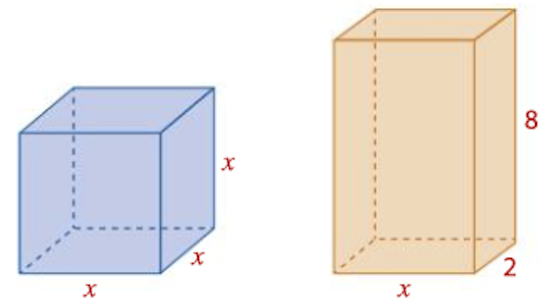
\includegraphics[scale=.7]{Ch 6/2}
\end{center}

Est-il possible de choisir $x$ de telle sorte que la boîte cubique ait une contenance supérieure à l'autre boîte ?

\end{Exercice}



\begin{Exercice}

Une entreprise fabrique des paniers. Elle peut en fabriquer jusqu'à $80$ par jour. Le coût de production en euros (matières premières, local, salaires\dots) de $x$ paniers est donné par : $C(x) = x^2 - 50x + 1000.$
Chaque panier est ensuite vendu $20$ € pièce.

\begin{enumerate}
    \item Quelle est la recette $R(x)$ de l'entreprise pour $x$ paniers fabriqués et vendus ?
    \item Quel est alors le bénéfice $B(x)$ de l'entreprise pour $x$ paniers fabriqués et vendus ?
    \item 
    \begin{enumerate}
        \item Montrer que $ B(x) = (x - 20)(50 - x).$
        \item Déterminer le nombre de paniers à fabriquer et à vendre quotidiennement pour que l'entreprise réalise un bénéfice.
    \end{enumerate}
\end{enumerate}

\end{Exercice}




}
